\section{Extended example}
\label{sec:imperative-balltracker}
To get a better feel for how a feedback control system works in practice, we will discuss a simple but interesting application of feedback control that uses the theory covered in the previous sections. In this section we show an imperative reference implementation. In the next chapter we will continue to use and refactor this application as we come up with an API for constructing and executing feedback systems. The application at hand is a port from the original implementation by Nikita Leshenko in Javascript, CSS and HTML \cite{nikital-balltracker}. We will however use Scala as our programming language and JavaFx for drawing the graphics on the screen. To get a feel of what this application is doing we strongly recommend to have a look at the online version\footnote{\url{http://nikital.github.io/pid/}} first before proceeding with this section!

The application consists of a flat surface on which a ball can move around. The goal is to move the ball from its initial position to the position on the surface that the user clicks on with the mouse. \Cref{fig:balltracker-initial} shows the ball in its initial state when the application starts. When the user clicks on the screen, the ball starts moving to that position as shown by \Cref{fig:balltracker-moving}. Besides the background and the ball, also the desired position, a dashed line between the ball and the desired position, the acceleration in both the $x$ and $y$ directions and a trail of previous positions are drawn (which are fading away over time). After some time the ball is at its desired position and waits there for a new position to navigate to, as is shown in \Cref{fig:balltracker-reached}. Notice that the desired position can also be updated while the ball is still moving, in which case it moves to the new and discards the old destination.

\begin{figure}
	\centering
	\begin{subfigure}[b]{0.80\linewidth}
		
\includegraphics[trim = 0mm 110mm 0mm 0mm, clip, width=\linewidth]{figures/BallTracker-initial.png}
		\caption{Initial}
		\label{fig:balltracker-initial}
	\end{subfigure}
	
	\begin{subfigure}[b]{0.80\linewidth}
		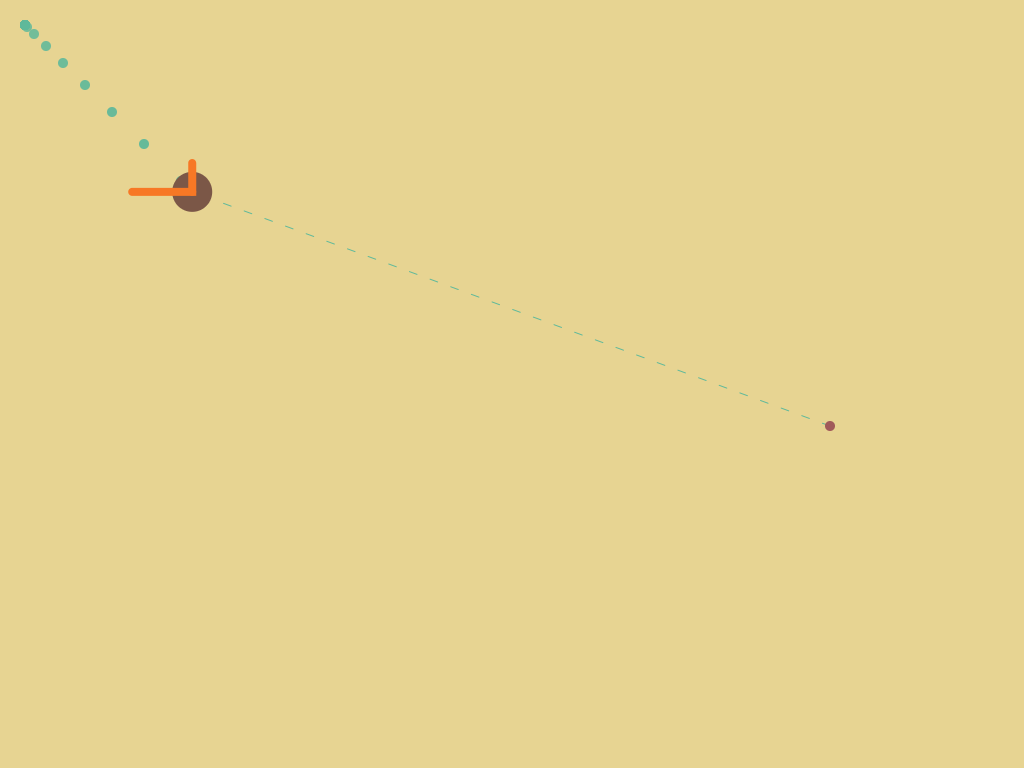
\includegraphics[trim = 0mm 110mm 0mm 0mm, clip, width=\linewidth]{figures/BallTracker-moving.png}
		\caption{Moving to desired position}
		\label{fig:balltracker-moving}
	\end{subfigure}
	
	\begin{subfigure}[b]{0.80\linewidth}
		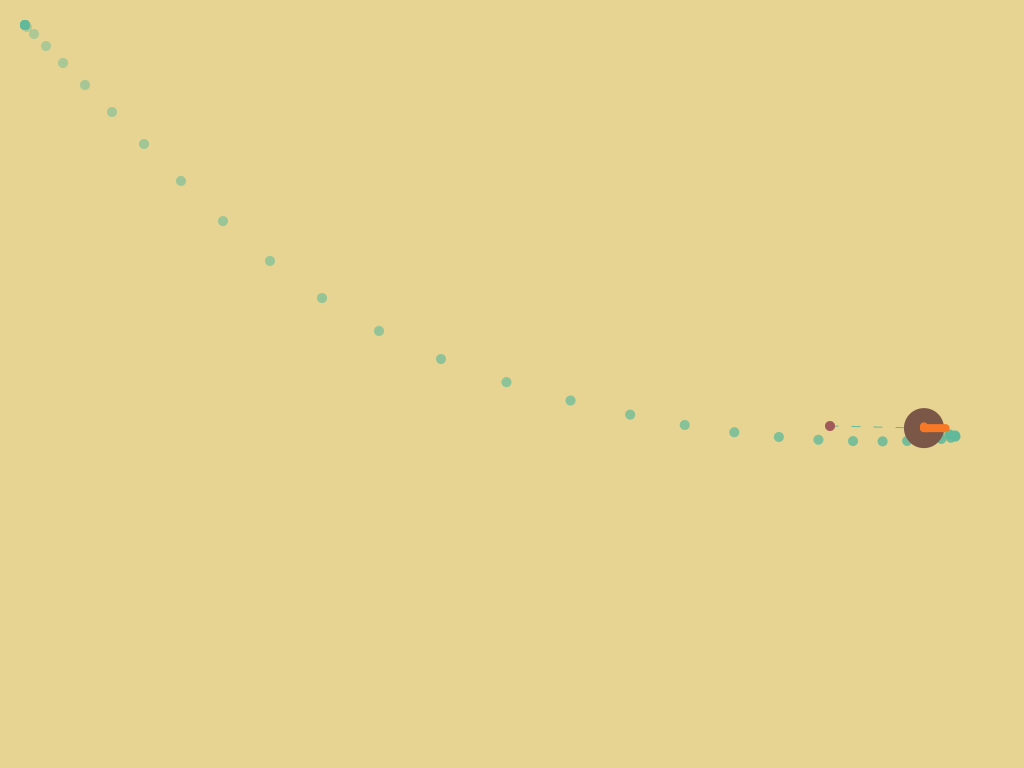
\includegraphics[trim = 0mm 110mm 0mm 0mm, clip, width=\linewidth]{figures/BallTracker-overshooting.png}
		\caption{Moving to desired position, overshooting a bit}
		\label{fig:balltracker-moving}
	\end{subfigure}
	
	\begin{subfigure}[b]{0.80\linewidth}
		
\includegraphics[trim = 0mm 110mm 0mm 0mm, clip, width=\linewidth]{figures/BallTracker-desired.png}
		\caption{Reached desired position}
		\label{fig:balltracker-reached}
	\end{subfigure}
	\caption{Ball movement}
	\label{fig:balltracker}
\end{figure}

In order to allow the ball to move in a natural way, we remind the reader of some basic equations from physics that describe the one dimensional motion of an object as a function of time (\Cref{eq:motion}). Here $x_t$, $v_t$ and $a_t$ are the ball's position, velocity and acceleration at time $t$ respectively. For two-dimensional motion we can combine two sets of these equations for both dimensions.

\begin{subequations}
	\begin{equation}
		x_t = x_{t - 1} + v_t \cdot \Delta t
	\end{equation}
	\begin{equation}
		v_t = v_{t - 1} + a_t \cdot \Delta t
	\end{equation}
	\label{eq:motion}
\end{subequations}

The implementation of these required pieces of physics can be found in \Cref{lst:ball-physics}. We first define a \code{Position}, \code{Velocity} and \code{Acceleration} as tuples of \code{Double} as well as some mathematical operations on the tuple type. The \code{Ball} class describes the state of the ball having a position, velocity and acceleration. A second constructor (\code{apply}) defines the initial position with no acceleration or velocity. The method \code{accelerate} on this class takes a new acceleration and calculates a new state for the ball according to \Cref{eq:motion}. Notice that we discard the $\Delta t$ term, since this will always be equal to 1. To keep track of the ball's previous positions we define \code{History} to be a queue of \code{Position}s.

\begin{minipage}{\linewidth}
\begin{lstlisting}[style=ScalaStyle, caption={Ball motion physics}, label={lst:ball-physics}]
type Position $=$ (Double, Double)
type Velocity $=$ (Double, Double)
type Acceleration $=$ (Double, Double)
type History $=$ mutable.Queue[Position]

implicit class Tuple2Math[X: Numeric, Y: Numeric](val src: (X, Y)) {
  import Numeric.Implicits._
  def +(other: (X, Y)) $=$ (src._1 + other._1, src._2 + other._2)
  def -(other: (X, Y)) $=$ (src._1 - other._1, src._2 - other._2)
  def *(scalar: X)(implicit ev: Y $=:=$ X) $=$ (scalar * src._1, scalar * src._2)
  def map[Z](f: X $\Rightarrow$ Z)(implicit ev: Y $=:=$ X): (Z, Z) $=$ (f(src._1), f(src._2))
}

case class Ball(acc: Acceleration, vel: Velocity, pos: Position) {
  def accelerate(newAcc: Acceleration) $=$ Ball(newAcc, vel + newAcc, pos + vel + newAcc) |\label{line:accelerate}|
}
object Ball {
  def apply(radius: Double) $=$ Ball((0.0, 0.0), (0.0, 0.0), (radius, radius))
}
\end{lstlisting}
\end{minipage}

The next step in creating this application is to design the feedback system itself (\Cref{fig:balltracker-diagram}). The \textit{system under control} here is of course the ball, from which at any point acceleration, velocity and position can be measured. Given that our \textit{setpoint} is equivalent to the position of where the ball should end up eventually, it makes most sense to define the \textit{control output} as the current position of the ball. From this it follows that the \textit{tracking error} represents the distance to be traveled before reaching the desired position. Depending on the distance, a controller can then decide how much it wants to speed up the ball by providing a new acceleration as the system's \textit{control input}. To get the ball's next position, this acceleration has to be integrated twice to get the ball's position after $\Delta t$ time.

To transform a distance into an acceleration, we can use the power of the PID controller. As discussed before, this controller is most commonly used because of its effectiveness and simplicity. For this use case it makes absolute sense to use the PID controller as well. The \textit{proportional controller} will look at the current distance to be traveled and comes up with some amount of acceleration. However, this acceleration will approach zero as the ball approaches its destination, causing it to keep its same velocity rather than slowing down. To prevent this, we need a strong \textit{derivative controller} that can counteract this velocity and slow down the ball as the distance is becoming smaller. For the purpose of looking back at previous distances we also add an \textit{integral controller} into the mix.

\begin{figure}[H]
	\begin{center}
		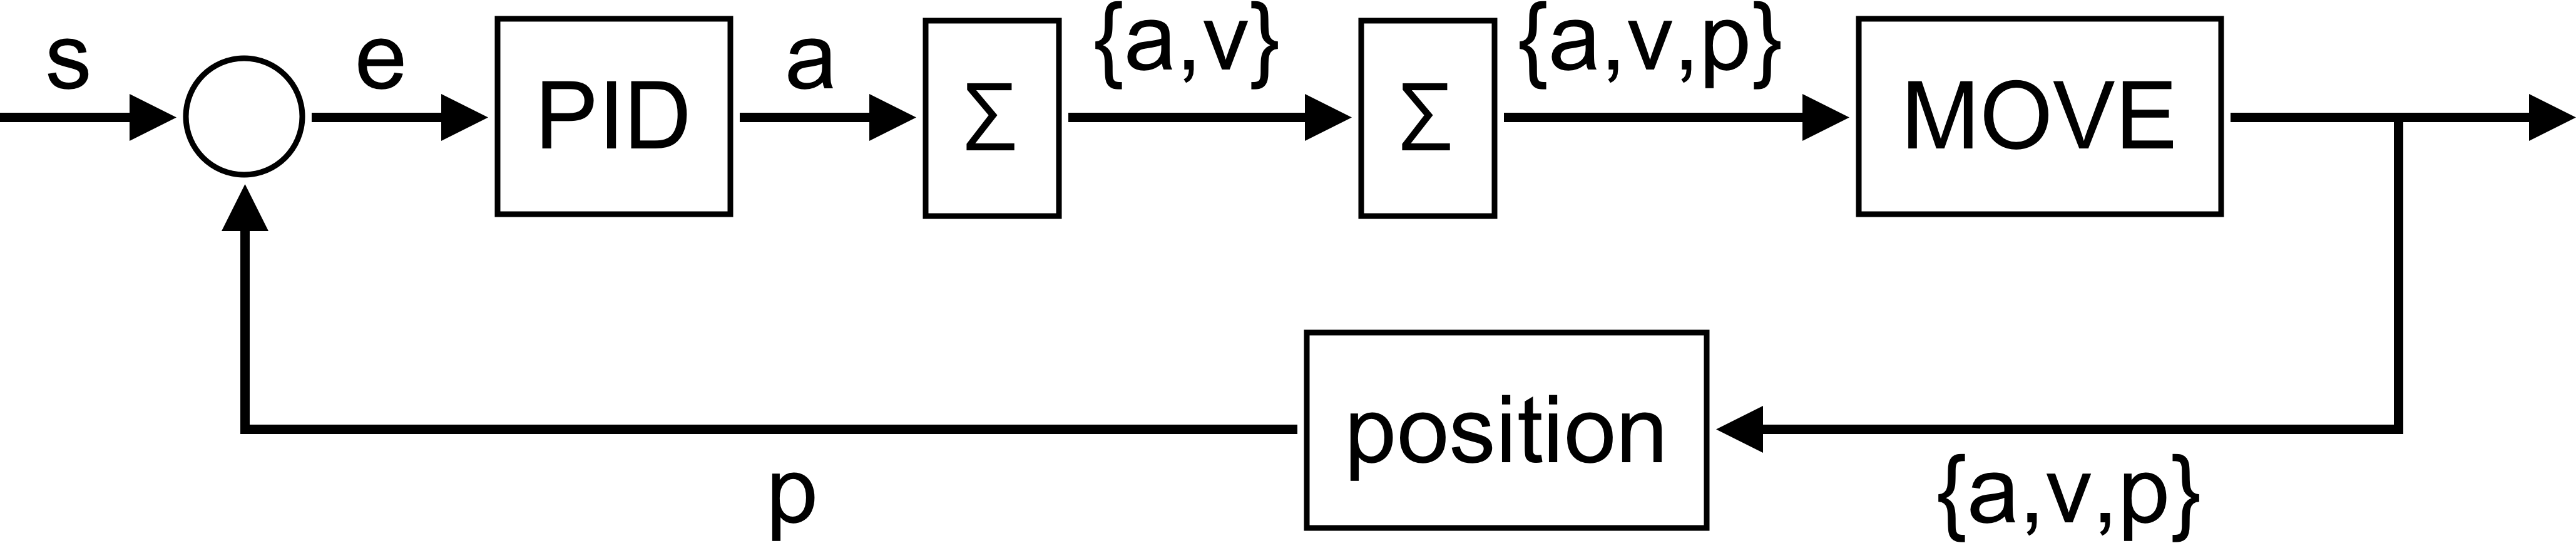
\includegraphics[width=0.85\textwidth]{figures/BallTracker-diagram.png}
	\end{center}
	\caption{Architecture of the ball movement control system}
	\label{fig:balltracker-diagram}
\end{figure}

Both the PID controller and the feedback system are implemented in \Cref{lst:ball-feedback}. After some initialization we define an iteration of the controller following \Cref{eq:proportional-control,eq:integral-control-discrete,eq:derivative-control} in the \code{pid} function on \cref{line:pid-function}. Again notice that this operates on the tuple types and uses the operators defined in \Cref{lst:ball-physics}. This function returns a new \code{Acceleration} which corresponds to the control input as described above.

The PID controller is then used in the construction of the feedback cycle (\cref{line:update}). It is first scaled down in such a way that it has an absolute maximum acceleration $0.2$, after which it is fed into the controlled system. This calls the \code{accelerate} function on the \code{Ball} (\Cref{lst:ball-physics} \cref{line:accelerate}), which calculates the ball's new velocity and position. The new state is then stored in the \code{ball} variable, which represents the latest control output. The rest of this function deals with managing the history and redrawing the application, which are considered not relevant for the implementation of the feedback system itself. The omitted code can be found in \Cref{app:ball-movement}.

Now that the feedback cycle is implemented, we can plug this in a JavaFx application that contains the canvas on which the application is drawn, as well as assigning the setpoint value and looping through the feedback cycle every 16 milliseconds. The code for this can be found in \Cref{app:ball-movement} as well.

Notice that with this feedback system we lack the notion of an external disturbance on the system under control. In this case there is none since the system is just the two \textit{sigma}s and the \textit{DRAW}. One could argue that the changing setpoint is kind of a disturbance, although this is by definition not the case. An example of an external disturbance on this particular system could be the terrain not being flat but rather containing hills and valleys. This would influence the ball's movement because of gravity, which would add a force in a third direction. For the sake of simplicity of this example we decided to not add this feature and stick with the flat terrain. We leave implementing this feature as an exercise to the reader.

\begin{minipage}{\linewidth}
\begin{lstlisting}[style=ScalaStyle, caption={Ball drawing}, label={lst:ball-feedback}]
var ball $=$ Ball(ballRadius)
var setpoint $=$ ball.position
var prevError, integral $=$ (0.0, 0.0)

// initializing history
// ...

def pid: Acceleration $=$ { |\label{line:pid-function}|
  val (kp, ki, kd) $=$ (3.0, 0.0001, 80.0)
  val error $=$ setpoint - ball.position
  val derivative $=$ error - prevError

  integral $=$ integral + error
  prevError $=$ error

  (error * kp + integral * ki + derivative * kd) * 0.001
}

def update(implicit gc: GraphicsContext): Unit $=$ { |\label{line:update}|
  val acceleration $=$ pid.map(a $\Rightarrow$ math.max(math.min(a, 0.2), -0.2))
  ball $=$ ball.accelerate(acceleration)

  // managing the history
  // ...

  // drawing all the elements
  // ...
}
\end{lstlisting}
\end{minipage}
